\subsubsection{Motor}
Als Motor wurde der STEPPERONLINE Nema 17 Schrittmotor\autocite{Schrittmotor} gewählt, der speziell für 3D-Drucker und CNC-Reprap-Maschinen konzipiert ist. Mit einem Drehmoment von 59 Ncm, einer Betriebsspannung von 24V, einem Strom von 2A und einem Schrittwinkel von 1.8 Grad pro Schritt gewährleistet er präzise Bewegungssteuerung. Das 4-Draht-Design und das beiliegende 1 Meter lange Kabel mit Verbinder ermöglichen eine einfache Integration in unsere Teststation. Dieser Schrittmotor ist optimal für DIY-Projekte und Anwendungen mit hohen Anforderungen an Präzision und Steuerung von Bewegungen.
\begin{figure}[H]
    \centering
    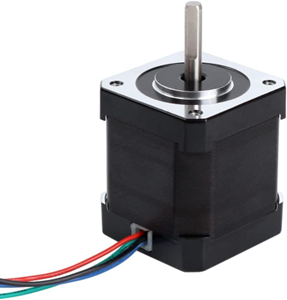
\includegraphics{image/schrittmotor.png}
    \caption{Schrittmotor}
    \label{fig:enter-label}
\end{figure}
Befestigung am Gyroskop und 5V Steuerung FETT:\\
\vspace{3mm}
Zuerst war geplant, den Ring im Gyroskop über eine Antriebsstange zu betreiben, dazu wäre ein 90° Umlenkung mit Zahnrädern notwendig gewesen. Da die Getriebe Stange über 30cm lang ist und nicht präzise zentriert ist, ist es schwierig, ein leicht gängiger Antrieb zu erhalten. Aus diesem Grund wird der Motor direkt an dem Linker Steher befestigt. \\
\vspace{3mm}
\begin{figure}[H]
    \centering
    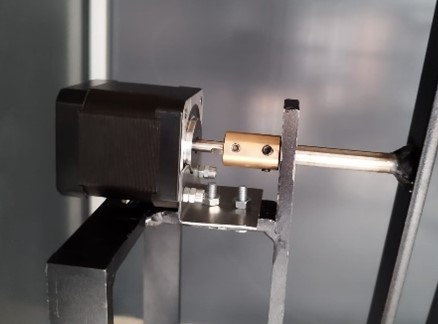
\includegraphics[scale=1.1]{image/motorgyros.jpg}
    \caption{Motor am Gyroskop}
    \label{fig:enter-label}
\end{figure}
\\
\vspace{2mm}
Die GPIO-Pins\label{sec: 5V} vom Raspberry Pi haben eine Ausgangsspannung von 3.3V. Für den Motor Treiber TB6600 wird aber eine Signalspannung von 5V benötigt. Mit einem NPN-Transistor und einem 2k2 Widerstand wird eine Ausgangsspannung von 5V erzeugt. Diese Zusammenschaltung wird auch Emitter Schaltung bezeichnet. Die Basis des bipolaren NPN-Transistors wird über einen Vorwiderstand mit dem Ausgangssignal eines GPIO-Pins vom Raspberry verbunden, während der Emitter mit dem 5V Ausgang vom Raspberry verbunden ist. Am Emitter ist zu gleich das Ausgangssignal mit nun 5V. Dieser wird mit dem Eingang vom Treiber verbunden. 